\documentclass[a4paper,12pt]{article}

\usepackage[english]{babel}
\usepackage[utf8x]{inputenc}
\usepackage{amsmath}
\usepackage{graphicx}
\usepackage{amssymb}
\usepackage{hyperref}
\usepackage{amsmath}
\usepackage{prettyref}
\usepackage{verbatim}
\usepackage[square,sort,comma,numbers]{natbib}
\usepackage[nohyphen]{underscore}
\usepackage[capitalise]{cleveref}
\usepackage[colorinlistoftodos]{todonotes}

\title{Finding Bot Accounts on Twitter via Tweets}
\author{David Tomassi, Somdutta Bose, Saja Alayadhi}

\begin{document}
\maketitle

\begin{abstract}
The goal is to detect bot accounts on Twitter via the granularity of tweets and their contents. Recently, we have seen the phenomena of ``Fake News'' and people's ability to buy bot accounts to respond to tweets and make them seem more popular. The significance of the project is to be able to see which accounts on Twitter are actually human. The data set we used is the MIB Dataset (http://mib.projects.iit.cnr.it/dataset.html) which has a genuine and bot account information and their respective tweets. We tokenized tweets and did an embedding (GloVe and Word2vec) of the tokens and then appended them together to be the input to our model. We investigate the effectiveness of different approaches using a single layer feed-forward neural network, multiple layer feed-forward neural network and Long short-term memory (LSTM). The results we present, show how accurate and precise the model is at determining if a Twitter account is a bot by the tweets.
\end{abstract}

\section{Introduction}
\label{sec:introduction}

Spam emails, advertisements, and communications in social media are a
common part of the internet and using these services. Detecting these
spam outlets has been a rich area of research
\citep{Cormack:2008:ESF:1454707.1454708,
DBLP:journals/corr/cs-CL-0009009, Androutsopoulos2006LearningTF,
Bickel:2006:DSF:2976456.2976477, Bratko:2006:SFU:1248547.1248644,
Solan:inproceedings, Cresci:2017:PSS:3041021.3055135, fameforsale2015,
INUWADUTSE2018496, FM2793, 8424744}.  With "Fake" news being spread
throughout social media \citep{NBERw25223} it has become imperative
that new methods and techniques be developed to address this
phenomenon. The focus on the social media platform Twitter has become
emergent \citep{8424744, FM2793, INUWADUTSE2018496,
Cresci:2017:PSS:3041021.3055135, fameforsale2015} as bot accounts
inflating the popularity of certian ideas has become common. Current
approaches to detect bot accounts use hand-engineered features which
can be troublesome to retrieve.

In this paper we introduce several different approaches to solve the
problem of detecting a bot account on Twitter by just a tweet. We use
different deep learning approaches using a feed-forward neural
network, an Long Short-Term Memory (LSTM) based architecture, and
Bidirectional Encoder Representations from Transformers (BERT) with
the goal of identifying a bot account by just a tweet. Since only a
tweet is required for classification, users do not have to be
encumbered with gathering a multitude of different data ranging from
number of followers, age of the account, and etc. This makes the
approach easier to use than previous methods.

The rest of the paper will be as follows: \cref{sec:methods} will
detail our approach, the results of our experiments will be described
\cref{sec:results}, we conclude in \cref{sec:conclusions}, in
\cref{sec:references} we discuss previous work, and in
\cref{sec:author-contributions} we detail each author's contributions.


\section{Related Work}
\label{sec:relatedwork}

In \cite{DeepNeuralNetworks}, the authors propose a deep neural network based on contextual long short-term memory (LSTM) architecture. They exploit both the content and metadata to detect bots at the tweet level. They extracted contextual features from user metadata and fed as auxiliary input  to LSTM deep nets processing the tweet text. They also proposed a technique based on synthetic minority oversampling to generate large dataset, suitable for deep nets training, from a minimum amount of labeled data. They demonstrated that with their architecture they achieved high classification accuracy (AUC \textgreater $96$\%) in separating bots from humans. When they applied the same architecture to account-level bot bot detection, they achieved nearly perfect classification accuracy (AUC \textgreater $99$\%). In \cite{DetectingSpamAccounts}, the authors propose a novel approach for distinguishing spam from no-spam social media post. They optimized a set of features independent of historical tweets. These tweets were available only for a short time on Twitter. Account features related to users were taken into account. They observed that an average automated spam account posted at-least  $12$ tweets a day at well defined periods. Their approach achieved a significant improvement on performance when compared to exiting spam detection techniques.

\section{Methods}
\label{sec:methods}

\subsection{Dataset} The dataset we will be using for our training and
evaluation will be the My Information Bubble (MIB) dataset
\citep{Cresci:2017:PSS:3041021.3055135}. It is a collection of genuine
and spam tweets from bot accounts. There are thousands of accounts
with millions of tweets. In one approach, we will split the dataset by accounts with a
$90$/$10$ split for training and validation data. In another approach, we will split the dataset into three sets (training, validation and testing). The split will be done by accounts level with a $80$/$20$ for training and testing data, then a split for the training data by $80$/$20$ for training and validation data. 

\subsection{Pre-Processing} We will pre-process the tweets in order to
normalize their format and reduce vocabulary size when we create an
embedding.

\subsubsection{Parsing} To parse the tweets, we will use three different ways depending on the embedding that will be mentioned in the next section. 

In the first approach, we split our tweet sentence on the basis of comma and strip the data of double quotes. We used a Word2Vec embedding \citep{Mikolov:2013:DRW:2999792.2999959} which decreases the dimensionality to $100$ to represent one word. We tried two other approaches, since this approach did not result in good results in terms of ``Accuracy''.

In one approach, we employ the
text-processing tool Ekphrasis
\citep{baziotis-pelekis-doulkeridis:2017:SemEval2} that will perform
tokenization, normalization and word segmentation. Using Ekphrasis
allows for a uniform format for the tweets and abstracts away
usernames and emojis which will decrease the vocabulary size that will
be used in the embedding. 

In another approach, we will preprocess the tweets based on the preprocessing script that is done by the creators of Global Vectors for Word Represention (GloVE) \citep{pennington-etal-2014-glove}. This will allow us to use the pre-trained word vectors for Twitter data provided by GloVE. 


\subsubsection{Embedding} Since our vocabulary size will be large as
the breadth of language, slang, and domain specific words is diverse.
Using a one-hot-encoding, would increase the dimensionality of the
input by a large margin. To overcome this obstacle, we used word embedding. We can either train the word embedding in our data or use a pre trained one. In this project we tried both of these approaches. In two approaches, we used a Word2Vec embedding \citep{Mikolov:2013:DRW:2999792.2999959} which decreases the dimensionality to $100$ to represent one word. In particular, we train a Word2Vec
model\footnote{https://radimrehurek.com/gensim/models/word2vec.html} on our tweets and use the embedding to encode them for input to the model. 

In another approach, we used the pre-trained GloVE specific in twitter data which encode the vocabularies in $100$ dimension vectors \footnote{https://nlp.stanford.edu/projects/glove/}. In particular, we used a set of the embedding from the pre-trained GloVE to encode our tweets to fed them as input to our model. 

\subsection{Pruning} We pruned tweets from our dataset that fall
outside the vocabularies that was learning from our Word2Vec model. With
the feed-forward neural network models, we limit the length of
the tokenized tweet as the input to the network has to be a fixed
sized. Tweets above this length threshold have been dropped from the
dataset and tweets below the threshold will be padded. While with the pre-trained Glove approach, we used zero vector to encode any vocabulary that falls outside the pre-trained Glove. 

\subsection{Feed-Forward Neural Network} For the first two approaches we have classified tweets in a feed-forward neural network
architecture. We have tried two different implementations with a single
hidden layer and multiple hidden layers.

\subsubsection{Single Hidden Layer} The single layered feed-forward
neural network are fully connected and have as input $20000$ sized
vector with a single hidden layer of $200$ neurons, and an output
layer with one neuron for prediction. The activation function for the
hidden layer will be the Rectified Linear Unit (ReLU) function and the
output layer will have the activation function as sigmoid to make the
prediction.

\subsubsection{Multiple Hidden Layers} The multiple hidden layered
feed-forward neural network are fully connected and have as input
$20000$ sized vector with three hidden layers of $200$ neurons each, and
an output layer with one neuron for prediction. Similarly, as the
single hidden layer feed-forward neural network, the activation
function for the hidden layers are ReLU and the output layer is sigmoid.

\subsection{Long Short-Term Memory (LSTM)}
In this model, we used pre-trained GloVE to encode the tweets text. So, the first part was preprocessing the tweets text to match the preprocessing for GloVE tweets, as mentioned in the parsing section. The labels were added to the dataset to recognize the ones from the genuine tweets’ dataset and the spam ones. The split of the data was done following the second approach mentioned in the dataset section. We developed the model using Keras framework  \citep{chollet2015keras}:
First layer was an embedding layer. This layer will take as an input : the maximum length of a tweet , which has been set in this approach to $140$, the number of vocabularies that we have, in this approach the counting was done for the training set, and the dimension of the dense embedding, in this approach is set to $100$. Since we used a pre trained Glove for the embedding, we provided this layer with the weights for the embedding and set them to be untrainable. 
The second layer is an LSTM layer with $100$ neurons and a $20$\% dropout. 
The final, output, layer has a single neuron for prediction with sigmoid function.


\subsection{Bidirectional Encoder Representations from Transformers (BERT)}
BERT is available for download on Github. The input file for this tool should be in a \textit{.tsv} file format. BERT accepts input (\textit{train.tsv} and \textit{dev.tsv}) in a certain format.  The input format that BERT accepts is given below:
\begin{itemize}
\item Column 1 is the id for a row.
\item Column 2 is a label for the row. This is an integer. These are classification labels that our classifier aims to predict.
\item Column 3 is a column of all the same letter {\textemdash}  this is a throw-away column that we need to include because the BERT model expects it.
\item Column 4 the text examples that we want to classify.
\end{itemize}
The file \textit{test.tsv} should be in another format. The format is given below:
\begin{itemize}
\item Column 1 is the id for a row.
\item Column 2 is the text that we want to classify.
\end{itemize}
There are four BERT ``base'' models which have different pre-trained weights. We picked ``cased'' and ``uncased''. These are use for different letter cases.
A script file is created to run BERT.  This script file contains the location of the input data files (\textit{.tsv}). It also contains entry to specify the location of BERT pre-trained weights.

On running this script file, we got an error. The error  is ``Assign requires shapes of both tensors to match.''. On searching for solution for this error, we found that this error may be caused because TensorFlow does not delete previous checkpoints. However, we have not found the correct solution to this problem.

\section{Results}
\label{sec:results}
\iffalse
Three metrics, in addition to classification accuracy, that are commonly required for a neural network model on a binary classification problem are:
\begin{itemize}
\item Precision: This is the ratio of the true positives to true positives and false positives (true positives / (true positive + false positive)). This is percentage of our results which are relevant.
\item Recall: This is the ratio of the true positives to true positives and false positives (true positives / (true positive + false negative)). This refers to the percentage of total relevant results correctly classified by our algorithm.
\item F1 score: F1 is a metric that takes into account both precision and recall. This number can be maximized to make our model better. F1 score = $2$ *(precision * recall)/(precision + recall)
ds

\end{itemize}
\fi
\subsection{Feed-Forward Neural Network}
Precision and recall are extremely important metrics to evaluate out model. Unfortunately, it is not possible to maximize both these scores at once. For problems for which both precision and recall are important, we can maximize the F1 score.

\subsubsection{Single Hidden Layer} Since we did obtain a high ``Accuracy'' with manually pre-processing the data, we used the tool Ekphrais for the same. Without Ekphrasis we got an accuracy of $36.08$\%. With Ekphrais, we got a accuracy of $87.3$\% for a single hidden layer feed-forward network.

\subsubsection{Multiple Hidden Layers} Without Ekphrasis we got an accuracy of $45$\%. With Ekphrasis we obtained and acuracy of $93.5$\% for multiple hidden layer
feed-forward neural network.

\subsection{Long Short-Term Memory}
This model achieved accuracy of $83.5$\% on the testing set and $89$\% on the validation set. Results of the modification in hyper-parameters and also the model architecture with pre-trained emending that all came with worse results are mention in the discussion section. 


\section{Discussion}
\label{sec:discussion}

\section{Conclusions}
This project aimed to classify a twitter account as a spam or not spam by using only a tweet text. We successfully got a good accuracy in two different approaches for the word embedding and tried to develop four models. The best accuracy obtained was $93.5$\%, from training using multiple hidden layer feed-forward neural network with Word2Vec embedding. 
\label{sec:conclusions}

%\section{References}
\label{sec:references}

\subsection{Email Spam Detection}

\subsection{Twitter Spam Detection}



\section{Author Contributions}
\label{sec:author-contributions}

\subsection{Saja Alayadhi}

\subsection{Somdutta Bose}

\subsection{David Tomassi}
\begin{itemize}
    \item Requesting Access to MIB Dataset
    \item Word2Vec Embedding
    \item Single Hidden Layered Feed-Forward Neural Network
    \item Multiple Hidden Layered Feed-Forward Neural Network
\end{itemize}


\bibliographystyle{splncs04nat}
\bibliography{main}
\section{Appendix}
\label{sec:appendix}

 \begin{figure}[h!]
  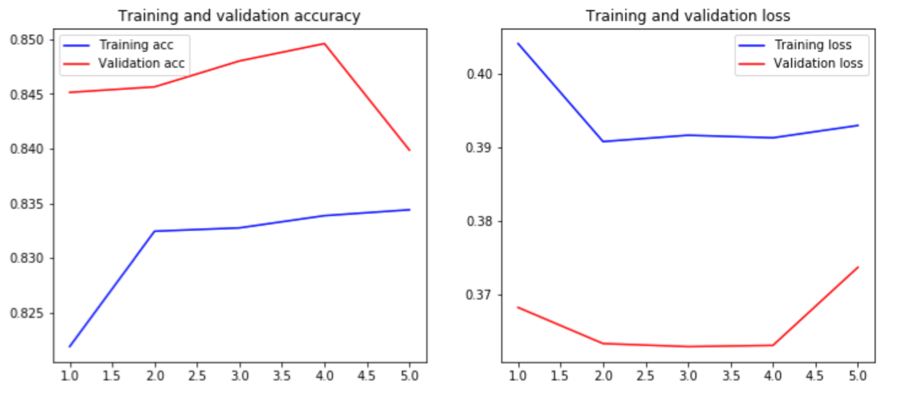
\includegraphics{multilayers.png}
  \caption{multiple hidden layered feed-forward neural network approach with pre-trained GloVE embedding where x-axis is the epochs and y-axis is: the accuracy on the left and the loss on the right}
  \label{fig:nnpre}
\end{figure} 

\begin{figure}[h!]
  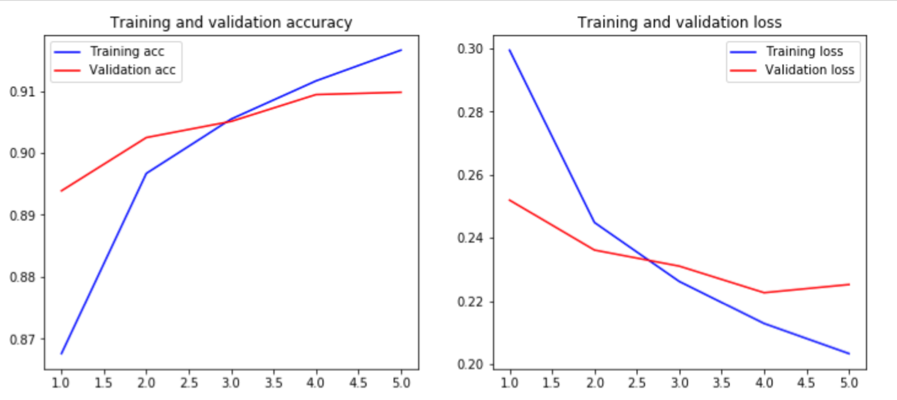
\includegraphics[width=\linewidth]{LSTM400.png}
  \caption{LSTM layer with 400 neurons where x-axis is the epochs and y-axis is: the accuracy in left and the loss on the right.}
  \label{fig:lstm400}
\end{figure}  

\begin{figure}[h!]
  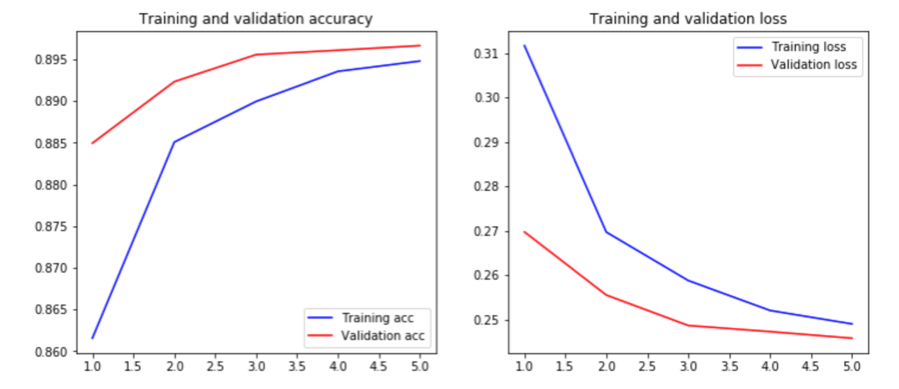
\includegraphics[width=\linewidth]{train90.png}
  \caption{LSTM model with 90\% for training data where x-axis is the epochs and y-axis is: the accuracy on the left and the loss on the right.}
  \label{fig:lstm90}
\end{figure} 

\begin{figure}[h!]
  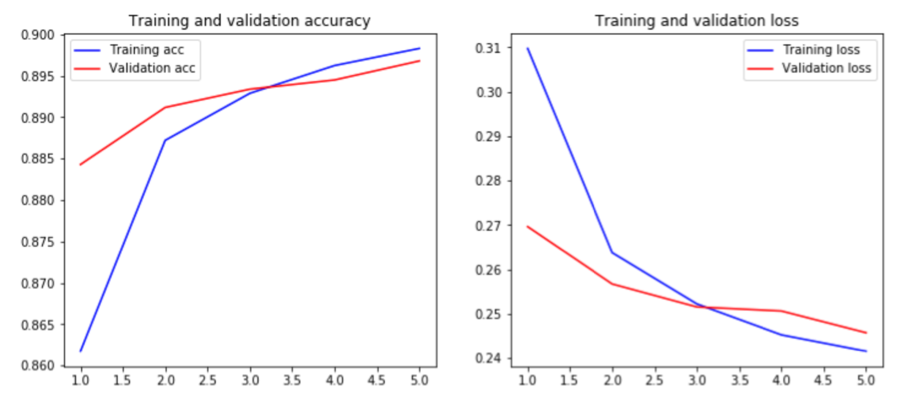
\includegraphics[width=\linewidth]{vocabChange.png}
  \caption{LSTM with embedding dictionary that doesn't have vocabularies from the validation data where x-axis is the epochs and y-axis is: the accuracy on the left and the loss on the right .}
  \label{fig:lstmvoc}
\end{figure} . 


\end{document}